\chapter{Introduction}

\section{Synthetic Data: Definition and Importance}
Synthetic data refers to artificially generated information that statistically mimics real-world datasets without directly copying individual records. Unlike anonymization or pseudonymization---which transform existing data---synthetic data generation creates entirely new samples from learned distributions, offering a fundamentally different approach to data privacy and availability challenges. According to Gartner, by 2030, synthetic data will completely overshadow real data in AI model training, underscoring the paradigm shift underway in how organizations source and utilize data \cite{figueira2022survey}.

The importance of synthetic data has grown exponentially in recent years, driven by three converging forces:

First, privacy regulations such as the General Data Protection Regulation \cite{gdpr2016regulation}, the California Consumer Privacy Act, the Health Insurance Portability and Accountability Act, and sector-specific mandates impose strict constraints on personal data usage. The GDPR alone applies to over 500 million EU citizens and mandates substantial fines---up to 4\% of annual global turnover---for non-compliance. Synthetic data provides a pathway to unlock analytical value while maintaining regulatory compliance, as synthetic records are not derived from any single individual and thus fall outside the scope of many personal data regulations.

Second, data scarcity remains a persistent challenge. Many domains suffer from insufficient data for machine learning applications, particularly for rare but critical events. In fraud detection, for instance, fraudulent transactions may constitute less than 0.5\% of all transactions, making it statistically difficult for models to learn meaningful patterns from the minority class. Synthetic data augmentation addresses this fundamental limitation by generating additional samples that preserve distributional properties while enriching underrepresented categories.

Third, the demand for collaborative analytics continues to grow. Organizations increasingly seek to share insights across institutional boundaries---between banks, hospitals, or research institutions---without exposing sensitive information. Synthetic data enables collaborative model development without data transfer, circumventing the legal, technical, and competitive barriers that prevent traditional data sharing. For example, multiple banks can train a joint fraud detection model using synthetic representations of each institution's data without any real customer records leaving their respective firewalls.

Recent advances in deep generative models---Generative Adversarial Networks (GANs) \cite{goodfellow2014gan}, Variational Autoencoders (VAEs) \cite{kingma2014vae}, and diffusion models \cite{ho2020ddpm}---have dramatically improved synthetic data quality, achieving near-indistinguishable fidelity on image and text domains. However, the application to structured tabular data, particularly in high-stakes domains like finance, remains comparatively underexplored and presents unique challenges that motivate this work.

\section{Motivation: Financial Sector Applications}
The financial services industry represents an ideal domain for synthetic data research due to its unique confluence of data sensitivity, regulatory pressure, and analytical requirements. The global financial services industry manages over \$26 trillion in assets, and the integrity of its data pipelines directly impacts economic stability and consumer welfare.

Financial records contain highly personal information---income, debt levels, transaction histories, creditworthiness assessments---whose exposure carries significant legal and reputational consequences. A single data breach in the financial sector costs an average of \$5.9 million as per the IBM Cost of a Data Breach Report, 2023. Unlike research datasets with informed consent, production financial data carries fiduciary obligations that preclude casual sharing or publication.

Financial institutions operate under overlapping regulatory frameworks:
\begin{itemize}
    \item \textbf{GLBA (Gramm-Leach-Bliley Act):} Mandates protection of consumers' nonpublic personal information, requiring financial institutions to explain their information-sharing practices.
    \item \textbf{PCI-DSS:} Governs payment card data handling with 12 core requirements for data security.
    \item \textbf{Basel III/IV:} Requires model validation on representative data, demanding that banks demonstrate model robustness across diverse economic scenarios.
    \item \textbf{Fair Lending Laws (ECOA, FCRA):} Necessitate bias auditing across demographic groups, requiring models to demonstrate fairness across protected categories such as race, gender, and age.
    \item \textbf{GDPR (EU):} Restricts cross-border data transfers and mandates data minimization principles.
\end{itemize}
These regulations simultaneously demand rigorous model validation while restricting the data available for such validation---a tension that synthetic data is uniquely positioned to resolve.

The critical analytical needs of the financial sector further motivate this work. Financial applications include:
\begin{itemize}
    \item \textbf{Fraud Detection:} Identifying rare malicious transactions (0.1--2\% prevalence). Global fraud losses exceeded \$32 billion in 2023.
    \item \textbf{Credit Risk Modeling:} Predicting default events (5--15\% prevalence) to set appropriate lending terms and capital reserves.
    \item \textbf{Anti-Money Laundering (AML):} Detecting suspicious activity patterns, where suspicious transaction reports represent less than 0.01\% of all transactions.
    \item \textbf{Algorithmic Trading:} Backtesting strategies on diverse market scenarios, including rare ``black swan'' events.
    \item \textbf{Insurance Underwriting:} Assessing risk for rare catastrophic claims.
\end{itemize}

Each application shares a common challenge: the events of greatest interest---fraud, default, market crashes---are precisely the rarest in historical data. Models trained on imbalanced datasets systematically underpredict these critical minority events, a phenomenon extensively documented in the imbalanced learning literature \cite{he2009imbalanced}.

\section{Why Tabular Data?}
We focus exclusively on tabular (structured) data for several compelling reasons:

Despite advances in deep learning for unstructured data, tabular formats dominate enterprise machine learning. Customer records, transaction logs, loan applications, and risk assessments are inherently structured. Gartner estimates that over 80\% of enterprise data resides in relational databases and spreadsheets. A 2023 Kaggle survey found that tabular data tasks account for approximately 65\% of all data science projects in industry settings.

Tabular data uniquely combines heterogeneous feature types:
\begin{itemize}
    \item \textbf{Numerical features:} Continuous (income, age, transaction amount) and discrete (count data, number of dependents).
    \item \textbf{Categorical features:} Nominal (occupation, state, transaction type) and ordinal (education level, credit rating grade).
    \item \textbf{Missing values:} Systematically or randomly absent entries that carry informational content (e.g., a missing employment field may indicate unemployment).
    \item \textbf{Complex constraints:} Business rules (loan amount $\leq$ property value), validity ranges (age $>$ 0), and inter-column dependencies (married status correlates with joint income fields).
\end{itemize}
This heterogeneity distinguishes tabular synthesis from image or text generation, where data types are homogeneous. As illustrated in Figure~\ref{fig:dataset_overview}, the datasets used in this study span a wide range of imbalance ratios and feature compositions.

\begin{figure}[H]
\centering
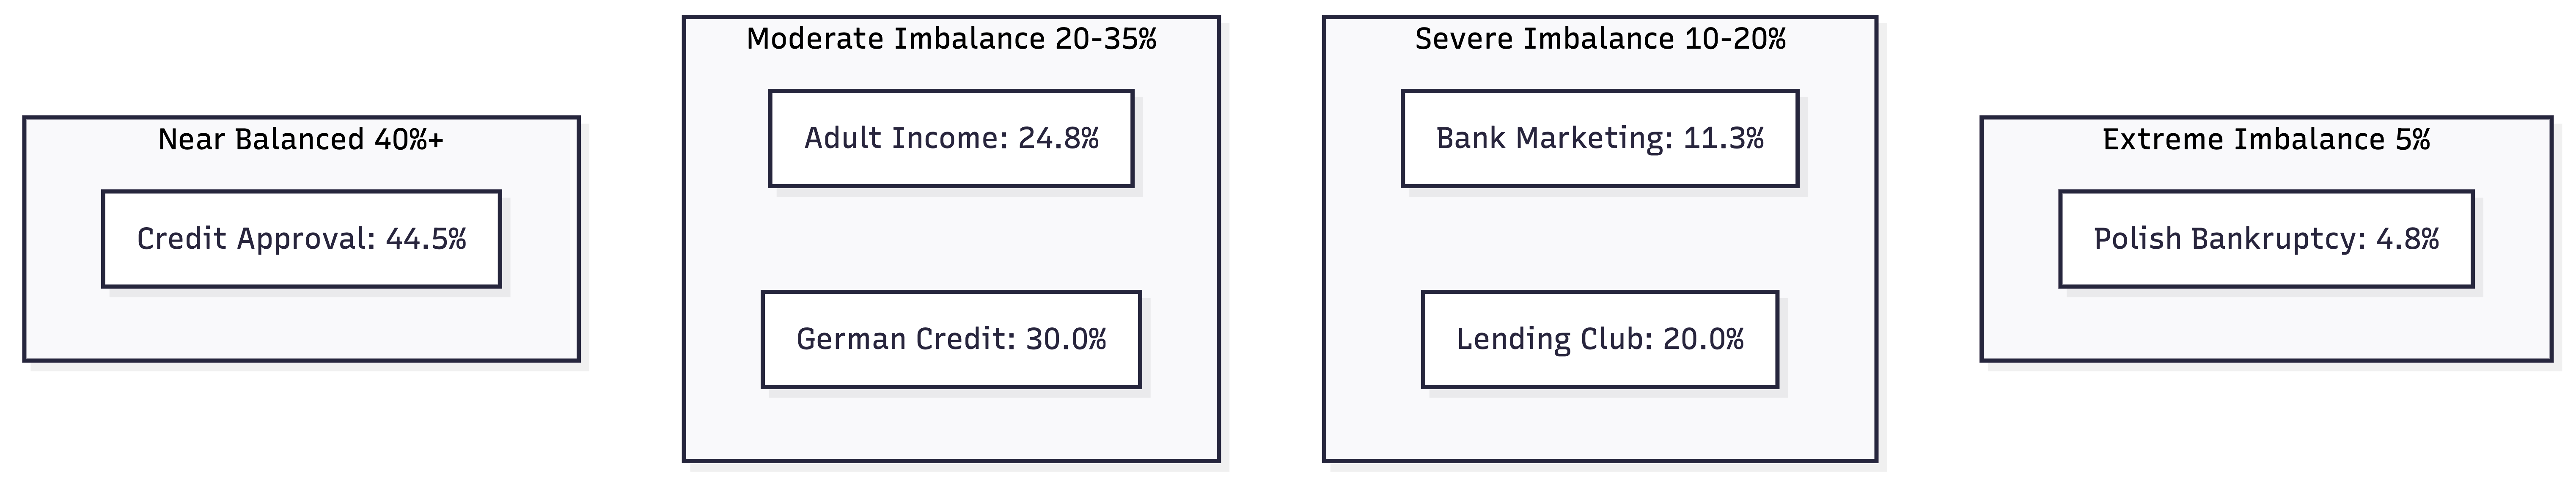
\includegraphics[width=\textwidth]{img/dataset_overview.png}
\caption{Overview of the six financial benchmark datasets used in this study, categorized by their class imbalance severity. Datasets range from near-balanced (Credit Approval at 44.5\%) to extreme imbalance (Polish Bankruptcy at 4.8\%).}
\label{fig:dataset_overview}
\end{figure}

Furthermore, tabular synthesis remains a significantly underexplored research area. Image synthesis has achieved remarkable results with models such as StyleGAN, DALL-E, and Stable Diffusion, as has text generation with GPT and LLaMA. Tabular synthesis lags significantly behind. Direct application of image-domain techniques fails on structured data, as we demonstrate empirically: TabDDPM \cite{kotelnikov2023tabddpm}, which applies diffusion directly to one-hot encoded tables, achieves KS statistics exceeding 0.80---indicating near-complete distributional mismatch. This failure occurs because one-hot encoded categorical features create sparse, discontinuous gradient landscapes that are incompatible with the smooth, continuous noise schedules used in standard diffusion processes.

Finally, tabular data underlies high-stakes decisions affecting individuals: loan approvals, insurance pricing, hiring recommendations, medical diagnoses. The quality of synthetic data directly impacts the fairness and accuracy of these decisions. A model trained on poorly synthesized data could systematically deny loans to qualified applicants or fail to flag fraudulent transactions, with material consequences for both consumers and institutions.

\section{Problem Statement and Research Gaps}
Despite significant progress in synthetic tabular data generation, a critical limitation persists: existing methods cannot control the class distribution of generated samples. This section examines the class imbalance problem in financial datasets, the limitations of current approaches, and the fundamental control gap that motivates this research.

\subsection{The class imbalance problem}
Financial datasets exhibit severe class imbalance, as documented across multiple benchmarks \cite{he2009imbalanced, chawla2002smote}:
\begin{itemize}
    \item Credit Card Fraud: Fraudulent transactions constitute only 0.1--0.5\% of the total.
    \item Loan Default: Defaulted loans represent 5--15\% of the portfolio.
    \item Company Bankruptcy: Only 3--8\% of companies in typical datasets are bankrupt.
    \item Suspicious Transactions (AML): Suspicious activity represents 0.01--1\% of all transactions.
\end{itemize}

Machine learning models trained on such data learn to predict the majority class, achieving high overall accuracy (e.g., 99\% by simply predicting ``not fraud'') while failing catastrophically on minority events---precisely the events of greatest business importance. This ``accuracy paradox'' means that standard evaluation metrics are misleading, and specialized metrics like minority-class F1-score, precision-recall AUC, and recall at fixed false-positive rates are essential.

\subsection{Limitations of existing approaches}
Traditional resampling methods have significant drawbacks:
\begin{itemize}
    \item SMOTE \cite{chawla2002smote} and its variants (Borderline-SMOTE, ADASYN) create interpolated samples that may lie outside the true data manifold, generating unrealistic feature combinations.
    \item Random undersampling discards valuable majority class information, reducing total training data and potentially removing important boundary examples.
    \item Neither approach generates truly novel samples; they merely redistribute or interpolate existing data points.
\end{itemize}

GAN-based methods such as CTGAN and TVAE also fall short:
\begin{itemize}
    \item Suffer from mode collapse \cite{salimans2016improved}, where the generator ``forgets'' minority modes of the distribution.
    \item Replicate the training class distribution without enhancement; generated data has the same imbalance as real data.
    \item No mechanism for post-hoc ratio adjustment---the user cannot request a specific minority ratio.
    \item Training instability makes reproducible results difficult to achieve.
\end{itemize}

Diffusion-based methods including TabDDPM and TabSyn present their own challenges:
\begin{itemize}
    \item TabDDPM \cite{kotelnikov2023tabddpm} fails on mixed-type data (KS $>$ 0.80), as direct diffusion on one-hot encoded features produces incoherent samples.
    \item TabSyn \cite{zhang2024tabsyn} achieves excellent fidelity (KS $\approx$ 0.10) by operating in a learned latent space but faithfully mirrors the training imbalance---if 5\% of training data is minority, approximately 5\% of synthetic data will also be minority.
    \item No existing diffusion-based method supports controllable class-conditional generation for tabular data.
\end{itemize}

\subsection{The control gap}
We identify a fundamental gap in the literature, confirmed through systematic review of 151 research papers across 10 categories:
\textit{No existing synthetic tabular data method enables practitioners to specify the desired class distribution during generation.}

This gap is particularly acute for financial applications, where balanced training data could significantly improve fraud detection, default prediction, and risk assessment. While Classifier-Free Guidance (CFG) \cite{ho2022cfg} has enabled remarkable control in image generation (enabling text-to-image models like Stable Diffusion \cite{rombach2022ldm} and DALL-E to produce highly specific outputs), its application to structured tabular data has remained entirely unexplored.

\section{Contributions}
This research makes the following contributions:

\textbf{1. Novel Application of Classifier-Free Guidance to Tabular Data.}
We introduce RE-TabSyn (Rare-Event Enhanced Tabular Synthesis), the first application of Classifier-Free Guidance (CFG) to tabular data synthesis. CFG, previously successful in image generation \cite{ho2022cfg}, enables controllable generation without auxiliary classifiers by jointly training conditional and unconditional models through a simple label dropout mechanism. This represents a fundamental advance in the tabular synthesis literature, opening a new research direction at the intersection of guided generation and structured data.

\textbf{2. Controllable Minority Class Generation.}
RE-TabSyn allows practitioners to specify target minority ratios via a single guidance scale parameter $w$. In our experiments, we boost minority representation from 4.8--44.5\% (original) to 44.8--50.2\% (generated), achieving near-balanced datasets on demand. This control is achieved at inference time without retraining the model, providing unmatched flexibility for downstream applications.

\textbf{3. Improved Minority Class Detection.}
We demonstrate that classifiers trained on RE-TabSyn synthetic data achieve a 3.1\% higher minority F1-score (0.472 vs.\ 0.458) than those trained on real imbalanced data---the first empirical evidence that guided synthetic data can outperform real data for minority detection tasks. This finding has profound implications for high-stakes applications where minority class detection is paramount.

\textbf{4. Comprehensive Financial Benchmark.}
We evaluate RE-TabSyn on six financial datasets spanning credit risk (German Credit, Credit Approval), income prediction (Adult Income), marketing response (Bank Marketing), loan performance (Lending Club), and corporate bankruptcy (Polish Bankruptcy). We provide systematic comparison against four baselines (CTGAN, TVAE, TabDDPM, TabSyn) across fidelity, utility, and privacy metrics, with statistical significance established across three random seeds (42, 123, 456).

\textbf{5. Conference Publication.}
The core findings of this research have been accepted for presentation at the \textbf{I2IT International Conference}, validating the scientific merit and novelty of the approach through external peer review. The paper titled ``\textit{Controllable Rare Event Synthetic Data Generation for Financial Tabular Data via Classifier Free Guidance}'' was accepted after rigorous review.

\section{Scope and Significance}
This section delineates the boundaries of the current research and articulates its practical, academic, and societal significance. The scope defines the specific problem domain and data characteristics addressed, while the significance highlights the broader impact across practice, research, and society.

\subsection{Scope}
This work addresses:
\begin{itemize}
    \item Binary classification tabular datasets with class imbalance (minority ratio from 4.8\% to 44.5\%).
    \item Single-table synthesis (relational/multi-table data is excluded from the current scope).
    \item Moderate dimensionality (tested on datasets with up to 64 features and up to 48,842 samples).
    \item Financial domain focus with broader applicability to healthcare, cybersecurity, and manufacturing.
\end{itemize}

\subsection{Significance}
RE-TabSyn enables financial institutions to:
\begin{itemize}
    \item Train more effective fraud detection models by generating balanced training data with realistic minority samples.
    \item Conduct bias auditing with balanced synthetic data across demographic groups without access to real protected-class data.
    \item Share data across organizational boundaries safely, enabling federated analytics without data exposure.
    \item Augment rare event datasets for improved stress testing and regulatory compliance.
\end{itemize}

From a research perspective, this work:
\begin{itemize}
    \item Bridges controllable image generation techniques (CFG) to the tabular domain for the first time.
    \item Establishes benchmarks for minority-aware synthetic data evaluation beyond simple fidelity metrics.
    \item Opens research directions in guided tabular synthesis, including multi-class control, continuous attribute conditioning, and privacy-guided generation.
\end{itemize}

Improved minority class detection directly benefits society:
\begin{itemize}
    \item \textbf{Consumers:} Better fraud protection, fairer credit decisions, and reduced false rejections.
    \item \textbf{Financial Institutions:} Reduced fraud losses, better risk models, and regulatory compliance.
    \item \textbf{Regulators:} Enhanced oversight capability through synthetic benchmarks for stress testing and fairness auditing.
\end{itemize}

\section{Organization of the Report}
The remainder of this report is organized as follows:
\begin{itemize}
    \item \textbf{Chapter 2: Research Analysis and Methodology} presents the formal problem formulation, mathematical foundations of baseline methods, and the detailed architecture and theoretical analysis of the proposed RE-TabSyn framework.
    \item \textbf{Chapter 3: Literature Review} surveys 151 peer-reviewed publications across generative models, tabular synthesis, privacy-preserving mechanisms, and evaluation frameworks, culminating in a gap analysis that motivates our approach.
    \item \textbf{Chapter 4: Implementation and Experimental Setup} describes the end-to-end pipeline, data preprocessing, model configurations, training procedures, and evaluation protocols.
    \item \textbf{Chapter 5: Research Outcomes} presents comprehensive results across fidelity, utility, privacy, and minority control metrics, with statistical significance analysis.
    \item \textbf{Chapter 6: Conclusion} summarizes key findings, discusses limitations, and presents concluding remarks.
    \item \textbf{Chapter 7: Future Scope} outlines promising research directions including architectural improvements, differential privacy integration, and extended synthesis capabilities.
\end{itemize}
